% XeLaTeX document
\documentclass[12pt,a4paper]{article}

% Редактируем: конфигурация, личные настройки: имя, название предмета и пр. для титульной страницы и метаданных документа здесь
\newcommand{\university}{Санкт-Петербургский политехнический университет Петра Великого}
\newcommand{\faculty}{Институт прикладной математики и механики}
\newcommand{\department}{Высшая школа прикладной математики и вычислительной физики}
\newcommand{\city}{Санкт-Петербург}
\newcommand{\docname}{Отчёт по лабораторной работе №5 \\ "ДВУСТОРОННИЕ МЕТОДЫ ДЛЯ ОБЫКНОВЕННЫХ ДИФФЕРЕНЦИАЛЬНЫХ УРАВНЕНИЙ"}
\newcommand{\subject}{Методы решения нелинейных задач}
\newcommand{\tutorname}{Фролов М.Е.}
\newcommand{\studentname}{студентка I курса магистратуры\\ Добрецова Е.В.\\}
\newcommand{\group}{5040102/40101}

% Не редактируем: используемые пакеты
% настройка кодировки, шрифтов и русского языка
\usepackage{fontspec}
\usepackage{polyglossia}

% рабочие ссылки в документе
\usepackage{hyperref}
\usepackage{listingsutf8}
\usepackage{listings}


% графика
\usepackage{graphicx}
\usepackage{tikz}
\usepackage{float} % force pictures position

% поворот страницы
\usepackage{pdflscape}

% качественные листинги кода
\usepackage{lstfiracode}

% отключение копирования номеров строк из листинга, работает не во всех просмотрщиках (в Adobe Reader работает)
\usepackage{accsupp}
\newcommand\emptyaccsupp[1]{\BeginAccSupp{ActualText={}}#1\EndAccSupp{}}
\let\theHFancyVerbLine\theFancyVerbLine
\def\theFancyVerbLine{\rmfamily\tiny\emptyaccsupp{\arabic{FancyVerbLine}}}

% библиография
\bibliographystyle{templates/gost-numeric.bbx}
\usepackage{csquotes}
\usepackage[parentracker=true,backend=biber,hyperref=true,bibencoding=utf8,style=numeric-comp,language=auto,autolang=other,citestyle=gost-numeric,defernumbers=true,bibstyle=gost-numeric,sorting=ntvy]{biblatex}

% установка полей
\usepackage{geometry}

% нумерация картинок по секциям
\usepackage{chngcntr}

% дополнительные команды для таблиц
\usepackage{booktabs}

% для заголовков
\usepackage{caption}
\usepackage{titlesec}
\usepackage[dotinlabels]{titletoc}

\usepackage{subcaption}

% разное для математики
\usepackage{amsmath, amsfonts, amssymb, amsthm, mathtools}

% водяной знак на документе, см. main.tex
\usepackage[printwatermark]{xwatermark}

\usepackage{dsfont}

\usepackage[normalem]{ulem} % для подчёркиваний uline
\ULdepth = 0.16em % расстояние от линии до текста выше/ниже


% Не редактируем: параметры используемых пакетов и не только
% настройки polyglossia
\setdefaultlanguage{russian}
\setotherlanguage{english}

% локализация
\addto\captionsrussian{
	\renewcommand{\figurename}{Рисунок}%
	\renewcommand{\partname}{Глава}
	\renewcommand{\contentsname}{\centerline{Содержание}}
	\renewcommand{\listingscaption}{Листинг}
}

% основной шрифт документа

\setmainfont{CMU Serif}[
Path = /Users/paks/Library/Fonts/,
UprightFont = cmunrm.ttf,
BoldFont = cmunrb.ttf,
ItalicFont = cmunbi.ttf
]






% перечень использованных источников
\addbibresource{refs.bib}

% настройка полей
\geometry{top=2cm}
\geometry{bottom=2cm}
\geometry{left=2cm}
\geometry{right=2cm}
\geometry{bindingoffset=0cm}

% настройка ссылок и метаданных документа
\hypersetup{unicode=true,colorlinks=true,linkcolor=red,citecolor=green,filecolor=magenta,urlcolor=cyan,
	pdftitle={\docname},
	pdfauthor={\studentname},
	pdfsubject={\subject},
	pdfcreator={\studentname},
	pdfproducer={Overleaf},
	pdfkeywords={\subject}
}

% настройка подсветки кода и окружения для листингов
\newenvironment{code}{\captionsetup{type=listing}}{}

% шрифт для листингов с лигатурами
\setmonofont{FiraCode-Regular.otf}[
	SizeFeatures={Size=10},
	Path = templates/,
	Contextuals=Alternate
]

% оформления подписи рисунка
\captionsetup[figure]{labelsep = period}

% подпись таблицы
\DeclareCaptionFormat{hfillstart}{\hfill#1#2#3\par}
\captionsetup[table]{format=hfillstart,labelsep=newline,justification=centering,skip=-10pt,textfont=bf}

% путь к каталогу с рисунками
\graphicspath{{fig/}}

% Внесение titlepage в учёт счётчика страниц
\makeatletter
\renewenvironment{titlepage} {
	\thispagestyle{empty}
}
\makeatother

\counterwithin{figure}{section}
\counterwithin{table}{section}

\titlelabel{\thetitle.\quad}

% для удобного конспектирования математики
\mathtoolsset{showonlyrefs=true}
\theoremstyle{plain}
\newtheorem{theorem}{Теорема}[section]
\newtheorem{proposition}[theorem]{Утверждение}
\theoremstyle{definition}
\newtheorem{corollary}{Следствие}[theorem]
\newtheorem{problem}{Задача}[section]
\theoremstyle{remark}
\newtheorem*{nonum}{Решение}

% настоящее матожидание
\newcommand{\MExpect}{\mathsf{M}}

% объявили оператор!
\DeclareMathOperator{\sgn}{\mathop{sgn}}

% перенос знаков в формулах (по Львовскому)
\newcommand*{\hm}[1]{#1\nobreak\discretionary{} {\hbox{$\mathsurround=0pt #1$}}{}}


% водяной знак для обозначения статуса документа
% \newwatermark[allpages,color=red!5,angle=45,scale=3,xpos=0,ypos=0]{DRAFT}
\begin{document}
% Не редактируем: Титульная страница (формируется автоматически из заданной конфигурации)
\begin{titlepage}	% начало титульной страницы

	\begin{center}		% выравнивание по центру

		\large \university \\
		\large \faculty \\
		\large \department \\[6cm]
		% название института, затем отступ 6см

		\huge \subject \\[0.5cm] % название работы, затем отступ 0,5см
		\large \docname \num \\ [5.1cm]
		% \large Тема работы\\[5cm]

	\end{center}


	\begin{flushright} % выравнивание по правому краю
		\begin{minipage}{0.25\textwidth} % врезка в половину ширины текста
			\begin{flushleft} % выровнять её содержимое по левому краю

				\large\textbf{Работу выполнила:}\\
				\large \studentname 
				\large {Группа:} \group \\

				\large \textbf{Преподаватель:}\\
				\large \tutorname

			\end{flushleft}
		\end{minipage}
	\end{flushright}

	\vfill % заполнить всё доступное ниже пространство

	\begin{center}
		\large \city \\
		  \large \the\year % вывести дату
	\end{center} % закончить выравнивание по центру

\end{titlepage} % конец титульной страницы

\vfill % заполнить всё доступное ниже пространство


% Не редактируем: Страница содержания (формируется автоматически из section, subsection и пр., указанных в content.tex)
% Содержание
%\tableofcontents
\newpage



% Редактируем: всё остальное: вступление, др. этапы, заключение, приложение
\section{Постановка задачи}
Необходимо на основе метода Рунге-Кутты построить двусторонние оценки решения следующей задачи Коши:
$$
\begin{cases}
	y'(x) = y cos(tx) \\
	y(0) = 1
\end{cases}
$$
Точным решением этой задачи является функция $y(x) = e^{\frac{sin(tx)}{t}}$.
\begin{figure}[H]
	\centering
	\begin{subfigure}{0.45\textwidth}
		\centering
		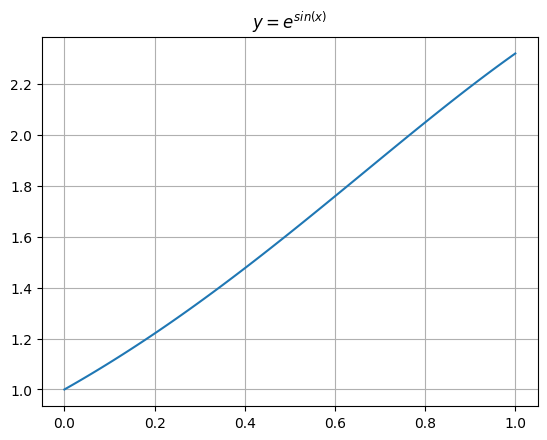
\includegraphics[width=\linewidth]{img/exact/exact1.png}
		\caption{$t = 1$}
	\end{subfigure}
	\hfill
	\begin{subfigure}{0.45\textwidth}
		\centering
		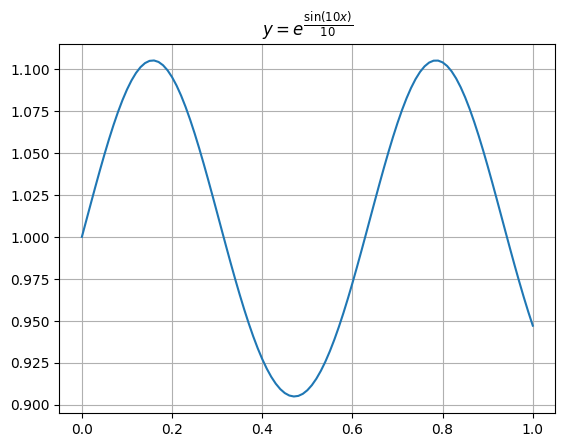
\includegraphics[width=\linewidth]{img/exact/exact2.png}
		\caption{$t = 10$}
	\end{subfigure}
	\caption{Точное решение задачи Коши при различных значениях параметра}
	\label{fig:two_graphs}
\end{figure}

\section{Цель работы}
Требуется на примере данной задачи исследовать эффективность двустороннего метода и сравнить его с методом Эйлера. Сравнение методоы нужно провести при различных значениях параметра $t$, рассмотрев сетки с шагом $h = 0.01, \: h = 0.005 \: \text{и} \: h = 0.0025$.

\section{Алгоритмы методов}
Поставлена задача Коши:
$$
\begin{cases}
	y'(x) = f(x, y) \\
	y(a) = y_0
\end{cases}
$$
Необходимо вычислить значения функции $y$ на множестве узлов $\{x_i\}_{i = 0}^n$, где $x_0 = a, \: x_n = b \: \text{и} \: x_i < x_{i + 1}.$
В данной лабораторной работе рассматриваются вычислительные схемы, относящиеся к группе методов Рунге-Кутты. Они основаны на использовании для перехода от узла $x_i$ к узлу $x_{i+1}$ определенного количества слагаемых из разложения функции $y$ в ряд Тейлора:
\[
y(x + h) = y(x) + h y'(x) + \frac{h^2}{2} y''(x) + \frac{h^3}{6} y'''(x) + \dots,
\]

где $x = x_i$, $h = x_{i+1} - x_i$.
\subsection{Метод Эйлера}
Метод Эйлера является простейшим из группы методов Рунге-Кутты. Его вычислительная схема выглядит следующим образом:
$$y(x + h) \approx y(x) + h f(x, y)$$
\subsection{Двусторонний метод Рунге-Кутты}
Двусторонний метод использует две независимые аппроксимации решения с различными коэффициентами, что позволяет получить верхнюю и нижнюю границы для значения $y(x)$ на каждом шаге.\\
\underline{Первый шаг метода: двусторонние оценки для $x_1$.}\\
Вычислим три промежуточных значения:
$$K_1 = f(x, y)$$
$$K_2 = f(x + h \alpha_2, y + h \beta_{21}K_1)$$
$$K_3 = f(x + h \alpha_3, y + h(\beta_{31}K_1 + \beta_{32} K_2)),$$
где $\alpha_2, \: \alpha_3, \: \beta_{21}, \: \beta_{31}, \beta_{32}$ - коэффициенты метода, обеспечивающие его порядок точности.
На основе этих значений строятся две различные оценки для $y(x_1) = y(x_0 + h)$:
\[
y^{(1)}(x + h) = y(x) + h (p_1 K_1 + p_2 K_2 + p_3 K_3)
\]
\[
y^{(2)}(x + h) = y(x) + h (\tilde{p}_1 K_1 + \tilde{p}_2 K_2 + \tilde{p}_3 K_3)
\]
Коэффициенты $p_1, \: p_2, \: p_3 \; \text{и} \; \tilde{p}_1, \tilde{p}_2, \: \tilde{p}_3 $ подобраны так, чтобы одна из формул переоценивала точное решение, а другая - недооценивала его.\\
В результате на первом узле $x_1$ получаем две границы для точного значения:
$$min(y^{(1)}, y^{(2)}) \leqslant y(x_1) \leqslant max(y^{(1)}, y^{(2)})$$
Таким образом, на первом узле мы получаем 2 приближённых значения.\\
\underline{Построение двусторонней оценки на i-м узле}\\
На каждом шаге строятся два новых значения на основе каждого из полученных на предыдущем шаге. Таким образом, на каждом следующем шаге количество аппроксимаций удваивается, следовательно, на i-м узле получается $2^i$ значений. Среди них выбираются максимальное и минимальное. Эти границы обеспечивают интервал, в который попадёт точка решения.

\section{Результаты}
\subsection{Визуализация двусторонних оценок}
Построим графики решения ДУ двусторонним методом Рунге-Кутты. Для наглядности выберем малое число узлов.
\begin{figure}[H]
	\centering
	\begin{subfigure}{0.45\textwidth}
		\centering
		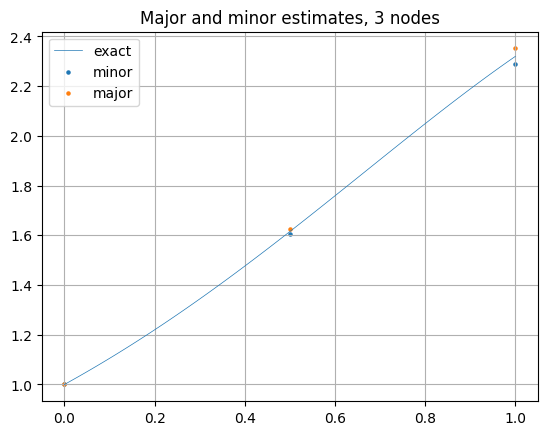
\includegraphics[width=\linewidth]{img/visualization/TwoSided3nodest1}
		\caption{$t = 1$}
	\end{subfigure}
	\hfill
	\begin{subfigure}{0.45\textwidth}
		\centering
		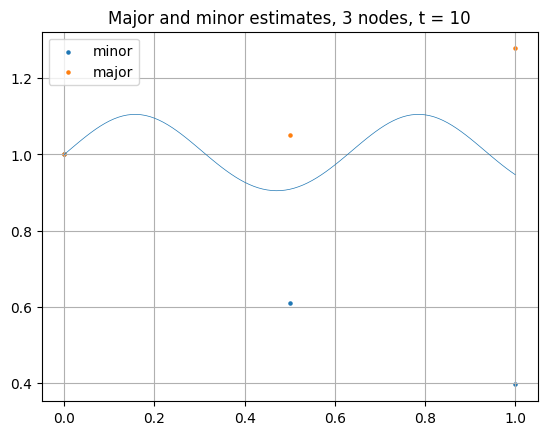
\includegraphics[width=\linewidth]{img/visualization/TwoSided3nodest2}
		\caption{$t = 10$}
	\end{subfigure}
	\caption{Двусторонние оценки при 5 узлах и различных значениях параметра}
	\label{fig:two_graphs}
\end{figure}

\begin{figure}[H]
	\centering
	\begin{subfigure}{0.45\textwidth}
		\centering
		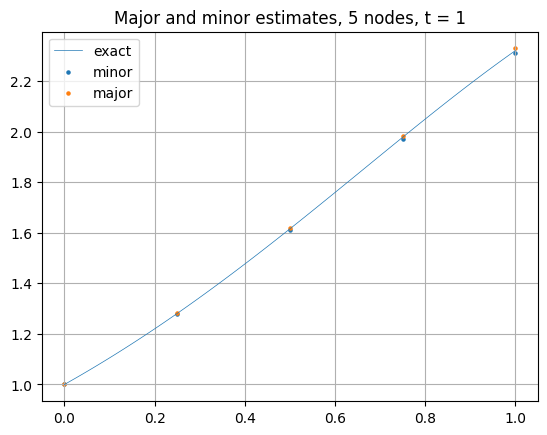
\includegraphics[width=\linewidth]{img/visualization/TwoSided5nodest1}
		\caption{$t = 1$}
	\end{subfigure}
	\hfill
	\begin{subfigure}{0.45\textwidth}
		\centering
		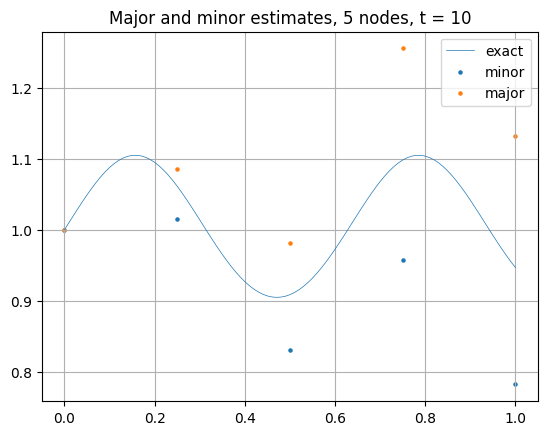
\includegraphics[width=\linewidth]{img/visualization/TwoSided5nodest2}
		\caption{$t = 10$}
	\end{subfigure}
	\caption{Двусторонние оценки при 5 узлах и различных значениях параметра}
	\label{fig:two_graphs}
\end{figure}

\begin{figure}[H]
	\centering
	\begin{subfigure}{0.45\textwidth}
		\centering
		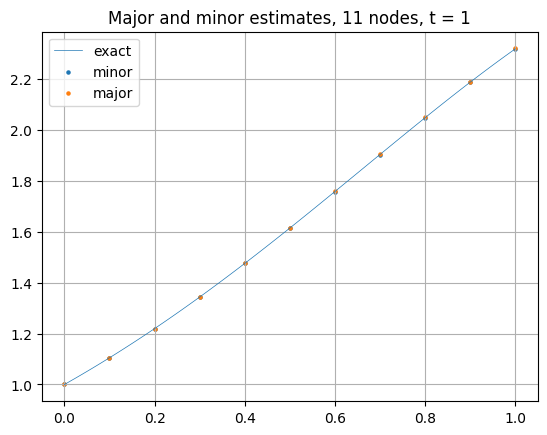
\includegraphics[width=\linewidth]{img/visualization/TwoSided11nodest1}
		\caption{$t = 1$}
	\end{subfigure}
	\hfill
	\begin{subfigure}{0.45\textwidth}
		\centering
		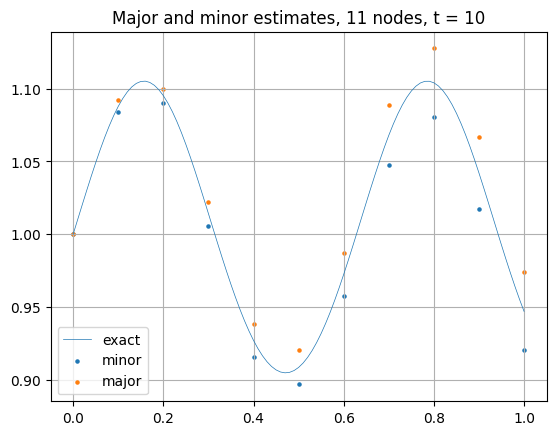
\includegraphics[width=\linewidth]{img/visualization/TwoSided11nodest2}
		\caption{$t = 10$}
	\end{subfigure}
	\caption{Двусторонние оценки при 11 узлах и различных значениях параметра}
	\label{fig:two_graphs}
\end{figure}

\subsection{Сравнение погрешностей метода Эйлера и двустороннего метода Рунге-Кутты}
\begin{figure}[H]
	\centering
	\begin{subfigure}{0.45\textwidth}
		\centering
		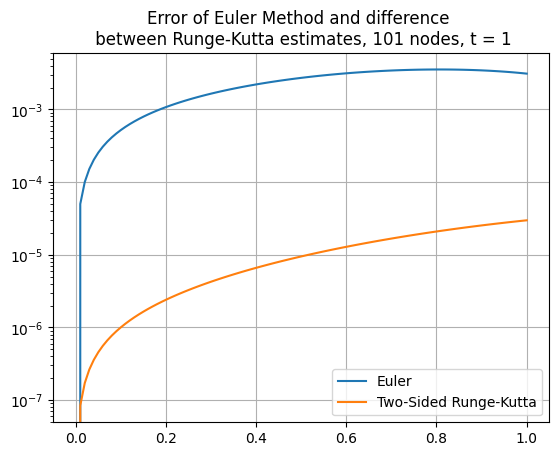
\includegraphics[width=\linewidth]{img/errorEulerAndDifferenceBtwEstimates/ErrEuDifRK11}
		\caption{$t = 1$}
	\end{subfigure}
	\hfill
	\begin{subfigure}{0.45\textwidth}
		\centering
		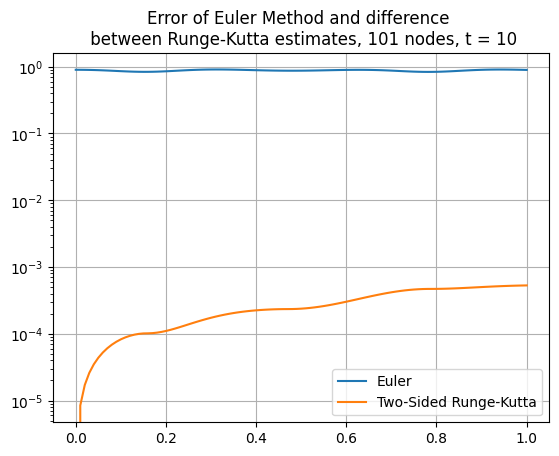
\includegraphics[width=\linewidth]{img/errorEulerAndDifferenceBtwEstimates/ErrEuDifRK12}
		\caption{$t = 10$}
	\end{subfigure}
	\caption{Двусторонние оценки при 101 узлах и различных значениях параметра}
	\label{fig:two_graphs}
\end{figure}


\begin{figure}[H]
	\centering
	\begin{subfigure}{0.45\textwidth}
		\centering
		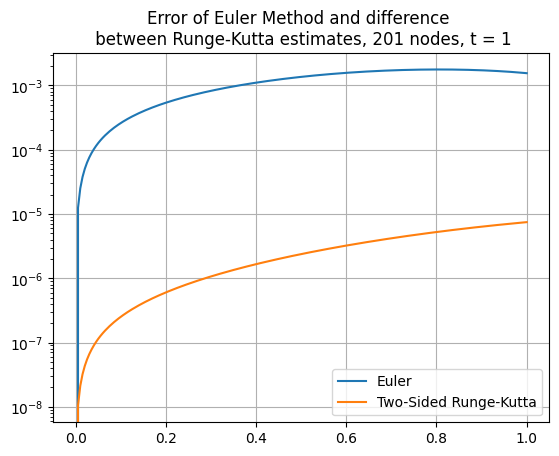
\includegraphics[width=\linewidth]{img/errorEulerAndDifferenceBtwEstimates/ErrEuDifRK21}
		\caption{$t = 1$}
	\end{subfigure}
	\hfill
	\begin{subfigure}{0.45\textwidth}
		\centering
		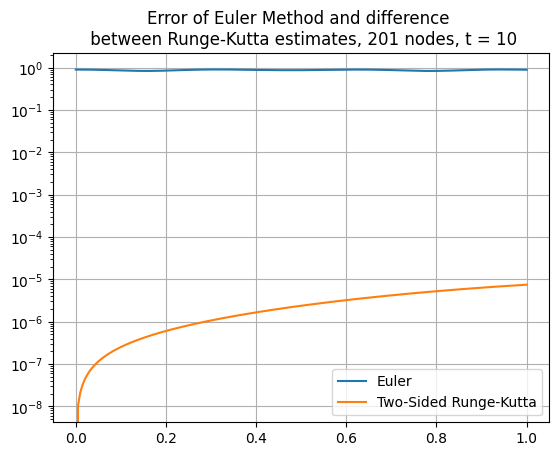
\includegraphics[width=\linewidth]{img/errorEulerAndDifferenceBtwEstimates/ErrEuDifRK22}
		\caption{$t = 10$}
	\end{subfigure}
	\caption{Двусторонние оценки при 201 узлах и различных значениях параметра}
	\label{fig:two_graphs}
\end{figure}

\begin{figure}[H]
	\centering
	\begin{subfigure}{0.45\textwidth}
		\centering
		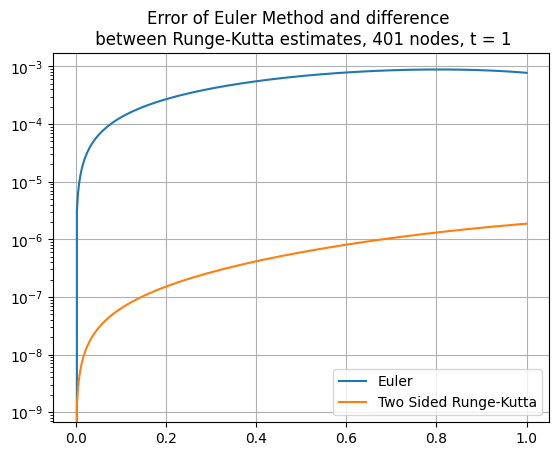
\includegraphics[width=\linewidth]{img/errorEulerAndDifferenceBtwEstimates/ErrEuDifRK31}
		\caption{$t = 1$}
	\end{subfigure}
	\hfill
	\begin{subfigure}{0.45\textwidth}
		\centering
		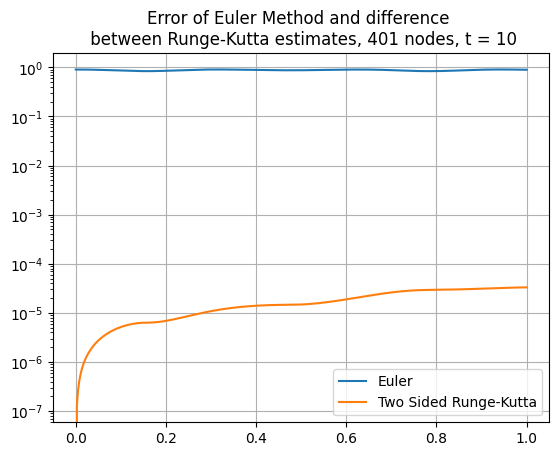
\includegraphics[width=\linewidth]{img/errorEulerAndDifferenceBtwEstimates/ErrEuDifRK32}
		\caption{$t = 10$}
	\end{subfigure}
	\caption{Двусторонние оценки при 401 узлах и различных значениях параметра}
	\label{fig:two_graphs}
\end{figure}


\section {Выводы}
% В ходе выполнения работы был реализован алгоритм двустороннего метода Рунге-Кутты, затем была исследована его эффективность и проведено сравнение метода Рунге-Кутты с методом Эйлера на примере двух задач Коши с известным точным решением.
% По результатам исследования можно заметить, что метод Рунге-Кутты превосходит метод Эйлера по точности. Если при решении задачи, точное решение которой имеет производную одного знака на данном отрезке, преимущество двустороннего метода Рунге-Кутты не так заметно (разница в 2-3 порядка), то на задаче, производная решения которой меняет знак, преимущество двустороннего метода Рунге-Кутты является неоспоримым, метод Эйлера к такой задаче практически неприменим из-за большой ошибки, а метод Рунге-Кутты даёт практически такие же результаты, как на задаче с производной одного знака.
% К недостаткам двустороннего метода Рунге-Кутты нужно отнести его трудоёмкость: на узле с номером $i$ требуется находить минимум и максимум среди $2^i$ значений, что требует больших вычислительных затрат.

В ходе выполнения работы был реализован алгоритм двустороннего метода Рунге-Кутты, проведено исследование его эффективности и выполнено сравнение с методом Эйлера на примере двух задач Коши с известным точным решением.

Анализ результатов показал, что метод Рунге-Кутты значительно превосходит метод Эйлера по точности. В случае задачи, точное решение которой имеет производную одного знака на заданном отрезке, преимущество двустороннего метода выражается в разнице порядка 2–3 десятичных разрядов. Однако при решении задачи, в которой производная изменяет знак, двусторонний метод Рунге-Кутты демонстрирует явное превосходство: метод Эйлера оказывается практически неприменим из-за высокой ошибки, в то время как метод Рунге-Кутты остаётся работоспособным и даёт значительно более точные результаты. При этом наблюдается небольшое снижение точности по сравнению с задачей, где производная не меняет знак.

Основным недостатком двустороннего метода Рунге-Кутты является его высокая вычислительная сложность. На узле с номером $i$i необходимо определять минимум и максимум среди $2^i$ значений, что значительно увеличивает затраты на вычисления.

% Не редактируем: Страница библиографии (формируется автоматически из книжек, указанных в refs.bib и пометок \cite{имя_источника} в тексте)
\newpage
\printbibliography[title=Перечень использованных источников]
\addcontentsline{toc}{section}{Перечень использованных источников}
\end{document}
